\documentclass[12pt]{report}
\usepackage{amsfonts}
\usepackage{amsmath}
\usepackage{amssymb}
\usepackage{amsthm}
\usepackage{cancel}
\usepackage{fullpage}
\usepackage{graphicx}
\usepackage{mathptmx}
\usepackage{parskip}
\usepackage{indentfirst}
\usepackage{xr}
\usepackage{xr-hyper}
\usepackage{paralist}
\usepackage{epstopdf}
\usepackage{wrapfig}
%\usepackage{hyperref}
%\usepackage{mcode}


\newcommand{\abs}[1]{\lvert#1\rvert}  % just makes it easier to do absolute values
\setlength{\parindent}{15pt}
\setcounter{topnumber}{10}
\setcounter{totalnumber}{10}

\pagestyle{empty}  % do not number the pages

\begin{document}
\rule{0pt}{1.1in}

%The command \rule[lift]{width}{height} produces a line of specified width and height, lifted above the location the amount "lift"
                % So, here we produce a space (0pt thickness) of height 2 in.

\begin{center}
{\Huge DARPA Robotics Challenge}

\vspace{0.4in}

\rule{2.1in}{0.1pt}

\vspace{0.5cm}


\textbf{A Major Qualifying Project\\
Submitted to the Faculty of\\
Worcester Polytechnic Institute\\
in partial fulfilment of the requirements for the\\
Degree in Bachelor of Science\\
in\\
Mathematical Sciences
and
Computer Science\\
By
\\*[12pt]}

Henrique Polido\\
\vspace{0.7cm}
\rule{2.1in}{0.1pt}
\vspace{0.5cm}


\end{center}
\vspace{0.5cm}  Date:  \today

\begin{center}
Approved: \vspace{0.5cm}
\end{center}

\hfill \underline{ \hspace{3in}}

\hfill Professor B.S. Arthur C. Heinricher~~

\hfill \underline{ \hspace{3in}}

\hfill Professor B.S. Michael A. Gennert~~

\vspace{ 0.5cm}

\noindent Keywords:\\
1. Inverse Kinematics \\
2. Robotics \\
3. Dynamic Programming

\setcounter{page}{1}
\begin{abstract}

This paper presents the Worcester Polytechnic Institute(WPI) and Carnegie Mellon University(CMU) team approach for competing on the DARPA Robotics Challenge (DRC) using the humanoid Boston Dynamics Atlas robot. An overview and analysis of the hardware and software architecture is described with emphasis on two of the challenges tasks, Wall and Drill. The realization of a double stance Inverse Kinematics(IK) full-body controller used for manipulation and its overall performance is elaborated. Moreover, an analysis for using Dynamic Programming optimization for robotic humanoid path planning is developed.


\end{abstract}

\newpage

\section*{Acknowledgements}
I would like to express my very great appreciation to my project advisers, Professor Arthur C. Heinricher and Professor Michael A. Gennert without whom this project would not have been possible. Their knowledge on the field and support to keep moving forward helped in the continuous development of the software for the Atlas robot. 

Special thanks for Worcester Polytechnic Institutes, and the great support it has had on my education, and the influence on my career. Honourable mentions towards Mathew DeDonato, Velin Dimitrov, and Perry Franklin. 

A huge thanks for my brother, Felipe Polido, to have introduced me into the project, and helped me with the many challenges of participating in a team, working through problems, and finding new solutions.

Thank you Carnegie Mellon University, with special consideration towards Eric Whitman, Chris Atkeson, and Siyuan Feng, for that without your help on the development on the controller, and many of the amazing motions that Atlas is able to achieve today. 

Lastly, thanks to the Nvidia Corporation for providing Worcester Polytechnic Institute for top of line graphical processing units. 

\newpage


\begin{center}
\includegraphics[scale=0.1]{images/atlas3.jpg}
\end{center}

\newpage
\setcounter{page}{1}
\renewcommand{\thepage}{\roman{page}}
\pagestyle{plain}

\newpage
\tableofcontents
\newpage
\renewcommand{\thepage}{\arabic{page}}
\setcounter{page}{1}
\pagestyle{plain}
%%%%%%%%%%%%%%%%%%%%%%%%%
\chapter{Introduction}
The work described in this report was done during the 2013-14 academic year in support of the WPI’s participation in the DARPA Robotics Challenge (DRC). WPI participated in two teams for the competition held in Homestead, Florida in December 2013.  For one of the teams, WPI faculty and staff joined a group headed by Drexel University.  For the other team, WPI partnered with faculty, staff, and students from Carnegie Mellon University. The work described here was done in support of the WPI-CMU team.  

There have been tremendous advances in solving the problem of controlling a humanoid robots \cite{eric_thesis}. Some of the mechanical problems have been solved by engineers at Boston Dynamics with the development of the Atlas robot. Key properties of the hardware, including sensors and actuators, are discussed in Section 3 below. 

Advances in mathematical modelling for the control of robotic systems have also made significant advances in recent years.  While the theory is well developed \cite{Deterministic_and_Stochastic}, limits in computational speed and power have kept the theory far short of practice.  One of the standard approaches for solving  the kind of optimization problems that arise in motion planning for a robot is the method of Dynamic Programming, originally developed by Richard Bellman. \cite{Deterministic_and_Stochastic} While the theory is powerful, the approach suffers from the curse of dimensionality \cite{random_sampling_dynamic_programming} and computational approaches fail for any realistically high-dimensional models.  The Atlas robot is very high dimensional, 28 independent hydraulic actuated joints. In addition, computational approaches to optimization can be very sensitive to model and sensor error. 

Any efficient computational approach must work with an approximate state space and an approximate controller and an approximation to the solution to the dynamic programming equations.  Atkison's \cite{random_sampling_dynamic_programming} and his co-authors have studied an approximation method that replaces a full optimization at each point in the state space with a simple comparison between the current “best” control strategy and a single, randomly generated, alternative.  Whitman \cite{eric_thesis} used this approximation technique but also studies an approach that separates the high-dimensional control problem for the Atlas robot into a family of low-dimensional (and so feasible) optimization problems and builds an approximate solution by integrating information from the many separate problems.  
Part of the work done in this project was on the implementation of approximation methods and techniques for speeding up the dynamic programming algorithm.  The approach is applied to the simplest model problem: the swing-up pendulum. \cite{eric_thesis} 

We will begin by describing some of the background, the motivation and the details in the Robotics Challenge, focusing on the properties and the limitations of the hardware.  The next section considers the software, starting at the overall infrastructure, and going into more detail about the manipulation software. 


\chapter{DARPA Robotics Challenge}
%\paragraph{The objective of this paper is to help the reader understand the current workings of the Carnegie Mellon’s University’s controller.}  
 
The DARPA Robotics Challenge (DRC) is a competition of teams developing robots capable of assisting humans in responding to natural and man-made disasters. The goal of the DRC is to design a robust robotic system that has mobility and dexterity in disaster zones, the ability to use tools designed for humans, and supervised autonomy.
 
Teams are spread in several tracks. Worcester Polytechnic Institute is in the Track C team, in which competed in the Virtual Robotics Challenge (VRC), and received funding for the Atlas robot.  

\section{Hardware}
\subsection{Atlas}
\begin{wrapfigure}{r}{0.3\textwidth}
  \begin{center}
    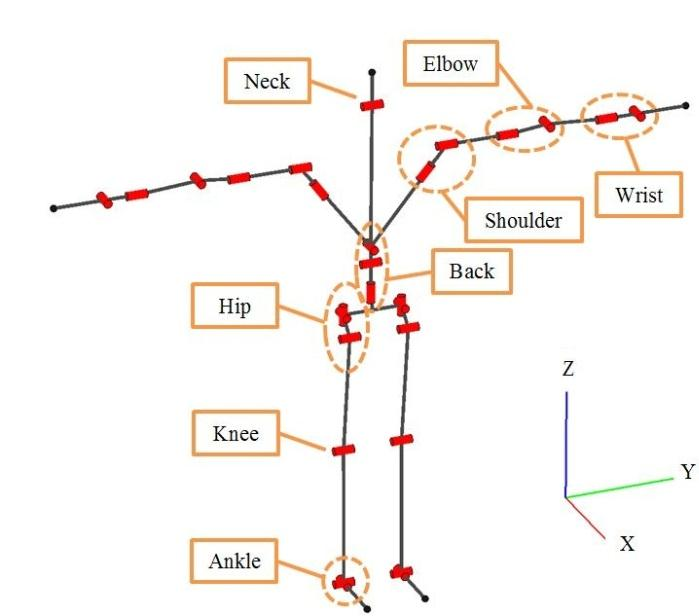
\includegraphics[scale=0.2]{images/atlas_joints.png}
  \end{center}
  \caption{Atlas' set of joints}
\end{wrapfigure}

As described by the Atlas Robot Operation and Maintenance Manual, "The Atlas robot’s on-board features include a real time computer, a hydraulic power pack, force/torque sensors, inertial sensing, and active thermal management. In addition to the integrated sensors, the Atlas robot comes equipped with the MultiSense-SL sensor head from Carnegie Robotics, and modular wrists"		

WARNER is 6 foot 2 inches tall and weighs approximately 330 pounds. The movement is powered by 28 hydraulically-actuated rotation joints, with a closed-loop position, velocity and force control. 

\subsection{Sensors}

Atlas is equipped with the following perception sensors:

\subsubsection{Carnegie Robotics Sensor Head}
\begin{wrapfigure}{r}{0.25\textwidth}
  \begin{center}
    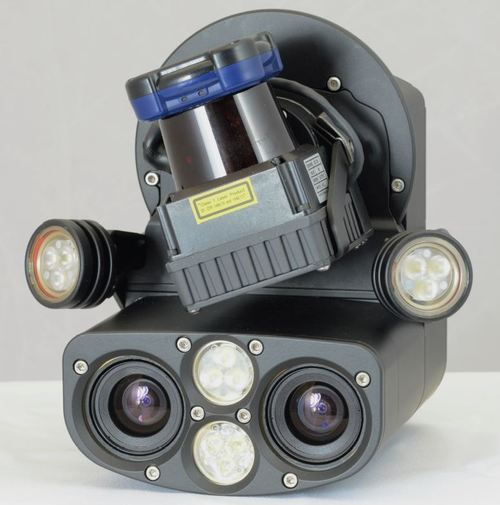
\includegraphics[scale=0.25]{images/sensorhead.jpg}
  \end{center}
  \caption{Multisense SL}
\end{wrapfigure}


The MultiSense SL is a tri-modal range sensor, providing laser range data, stereo range data, and video output stream. The device supply the majority of perceptual data used for tele-operation as well as automated control. 

The apparatus brings together a Hokuyo UTM-30LX-EW laser, which output 43,000 points per second, and a Carnegie Robotics MultiSense S7 high resolution stereo camera, with a 4 megapixels on each side.  On-board processing handles image rectification, stereo data processing, time synchronizing of laser data with a spindle encoder, spindle motor control, and lighting timing. \cite{multisense-sl}

\subsubsection{Situational awareness cameras}

Two situational awareness cameras are placed just below the head of the robot, providing a wide range view of the workspace.

\begin{figure}[ht]
\begin{center}
\begin{minipage}[b]{0.4\linewidth}
\centering
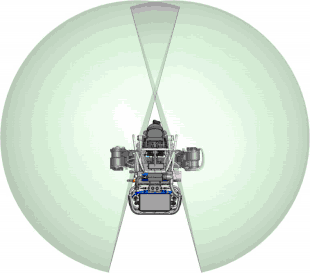
\includegraphics[width=\textwidth]{images/sitcamFOV.png}
\caption{Top-down view of the robot, display range of view}
\label{fig:figure1}
\end{minipage}
\hspace{0.5cm}
\begin{minipage}[b]{0.4\linewidth}
\centering
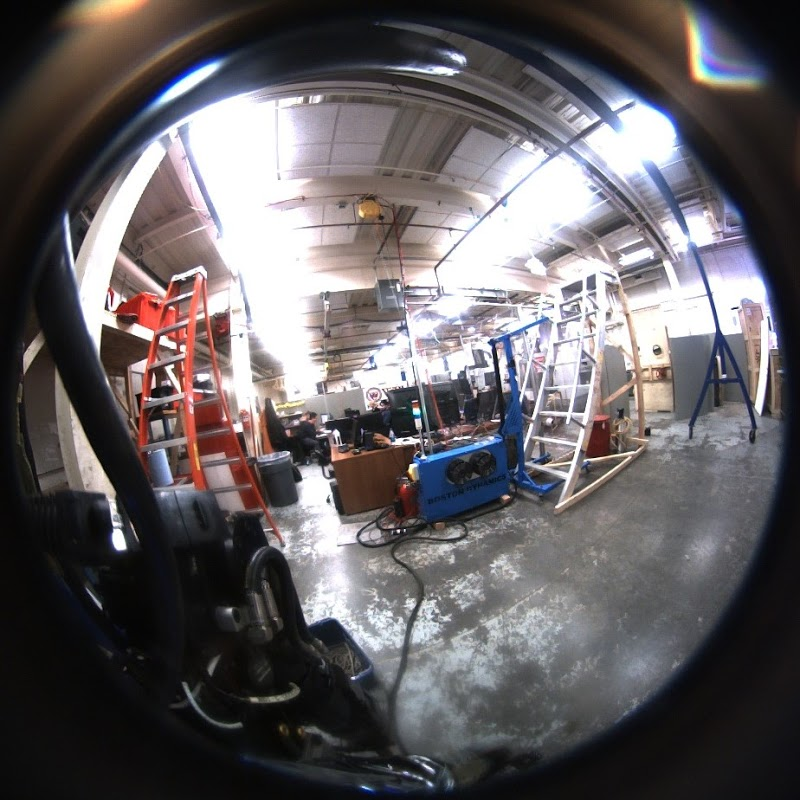
\includegraphics[width=\textwidth]{images/fisheye.jpg}
\caption{View of the camera}
\label{fig:figure2}
\end{minipage}
\end{center}
\end{figure}

\pagebreak


\subsubsection{Atlas Control Parameters}
There exists several controller parameters that is hidden to the developer that controls the hydraulic joints. We let $q$, $qd$ and $f$ be the senses position, velocity, and torque respectively. And we let $q_d$, $qd_d$, and $f_d$ be the desired position, velocity, and torque for each joint.

We create the following variables to help control the desired torque control:

\begin{itemize}
\item $k_{q_p}$: Position error gain, in $\frac{N \cdot m}{rad}$.
\item $k_{q_i} $: Integral of position error gain, in $\frac{N \cdot m}{rad \cdot s}$.
\item $k_{{qd}_p}$: Derivative error gain, in $\frac{N \cdot m}{\frac{rad}{s}}$.
\item $k_{f_p}$: Proportional force feedback gain.
\item ${ff}_{qd}$: Feedforward velocity gain.
\item ${ff}_{{qd}_d}$: Feedforward desired velocity gain.
\item ${ff}_{f_d}$: Feedforward desired force gain.
\item ${ff}_{const}$: Constant force term.
\end{itemize}

And use them accordingly: 
\begin{align*}
k_{q_p} &\cdot ( q_d - q ) &+\\
k_{q_i} &\cdot 1/s * ( q_d - q ) &+\\
k_{{qd}_p} &\cdot ( {qd}_d - qd ) &+\\
k_{f_p} &\cdot ( f_d - f ) &+\\
{ff}_{qd} &\cdot qd &+\\
{ff}_{{qd}_d} &\cdot qd_d &+\\
{ff}_{f_d} &\cdot f_d &+ {ff}_{const}
\end{align*}

\subsection{Robotiq Hand}

The robot gives the option of interchanging the hands. DARPA offered two primary options: the iRobot© hands, and the Sandia© hands. While both options are from known companies in the industry, neither provided the power, nor robustness necessary to complete the high demanding tasks of the DRC. These hands were designed to perform precision tasks, such as picking up a coin, or a fist-sized rock, but not to handle a power tool, or hold the Atlas robot while climbing up a ladder. The team chose an alternative end-effector developed by Robotiq©, a 3-Finger adaptive industrial robot gripper, which provided a much stronger grip. 

\section{Software}
The software developed my WPI and CMU are mostly written in C++, with small parts written in Python. 

\subsection{DBI Behaviours}
Boston Dynamics provided predefined behaviours for Atlas that allow for basic performance like balancing and walking. Transitions between behaviours can occur manually or automatically, and follow a pre-determined state-machine.

\subsubsection{Manipulate}
\begin{wrapfigure}{r}{0.3\textwidth}
  \begin{center}
    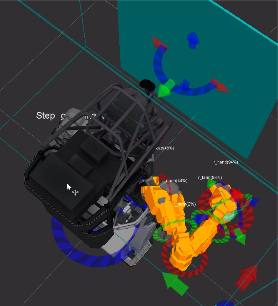
\includegraphics[scale=0.5]{images/align_to_wall.png}
  \end{center}
  \caption{Rviz within ROS}
\end{wrapfigure}
In manipulation mode the user can control all the joints above the torso, and basic control of the pelvis orientation and height. The legs and overall balance are controlled by the Boston Dynamics controller embedded in the firmware.

The manipulation mode has a wide range of motion if the pelvis position and orientation is controlled together with an inverse kinematics solver for the joints, but can be unpredictable. The robot back joint that controls forwards and backwards motion was originally to weak, is unable to maintain position in certain configurations. The failure of this joint may compromise any given manipulation task.

Lastly, in this mode the user has the option to input any additional weight from objects in the hand to help the controller maintain balance.


\subsubsection{Walk}
 \begin{wrapfigure}{r}{0.3\textwidth}
  \begin{center}
    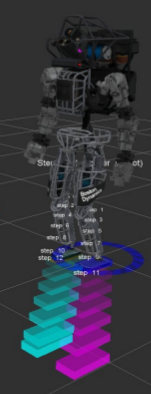
\includegraphics[scale=0.4]{images/step_gui.png}
  \end{center}
  \caption{The planned steps for the robot walking forward and to the left}
\end{wrapfigure}


Boston Dynamics walking behaviour works by the user providing a sequence of steps parameters, which include the step duration, sway duration, swing height, lift height, and step end distance.   

The WPI team developed an additional interface for Rviz so that the robot operator is able to specify a final desired feet positions for the robot, and the software produces all the intermediate steps. It took some trial-and-error testing to figure out what the maximum step size is, and the program does not account for any debris on the floor.

Although it could be automated, it is also usually required for the operator to additionally modify the final two steps such that they are further apart, thus providing a larger support polygon for manipulation. 

\subsection{Architecture}

The system architecture was setup in three major components: 

\subsubsection{Atlas}
The control loop inside the Atlas robot is inaccessible by the team, and can only be interfaced through a C++ API provided by Boston Dynamics. The API works by connecting to the robot through an IP address, queuing packets received from the robot, and sending back responses. 

\subsubsection{Field Computer}
The Field Computer is designed to handle the team programmed controller logic of the robot, either being a full body controller, or using the predefined behaviours given by Boston Dynamics. This is also where high-bandwidth perception and autonomous algorithms function.

If the Field Computer fails to send a new command to the robot within 0.2 milliseconds, the robot will automatically shutdown. 

Lastly, it is responsible for sending and receiving high level commands from the Operational Command Unit.

\subsubsection{Operational Command Unit (OCU)}

The Operational Command Unit(OCU) is the interface between the operator and the field computer. Our team relied on multiple operators working in individual OCU computers networked together. From the OCU the operators have to evaluate the robot situation, reason, and execute the desired tasks.

%\subsubsection{Motion controller}
%The motion controller is responsible for controlling the joints of the robot. 

%Most of the math executed is done with the help with Eigen, a C++ template library for linear algebra. 

\subsection{Network}

DARPA structured a predictable, but limited bandwidth communication between the field computer and the OCU. The network quality varied every 60 seconds between a $1000 \frac{kb}{s}$ with a $100ms$ round trip delay, and a $100 \frac{kb}{s}$ with a $500ms$ round trip delay. This setup is to incentive the teams to perform the tasks autonomously.

The challenge used a Mini Maxwell \cite{minimaxwell}, a network emulation system, to enforce the bandwidth limitations. The exact configurations of the Maxwell was never revealed, but whenever the bandwidth limitations was surpassed, packets seemed to be LIFO queued, sometimes causing images from the video stream to come out of order. 

\subsection{ROS}

Robot Operational System (ROS) is a messaging messaging software that allows for remote procedure calls (RPC) through pre-defined message definitions. The basics of the framework allows for nodes to publish messages on given names, and any other piece of software on the network can listen to the message by knowing the name of published message. 

For example, an important piece of software, TF, listens to messages about the robot joint states, and with additional information about kinematic model, publishing information about the transformation matrices between each frame of reference between on the body. 

\subsubsection{MoveIt!}
MoveIt! is a software developed with ROS to help robot developers control the robot. It contains a inverse kinematics solver that can interface with Atlas, but prevents two containing limitations: 
\begin{inparaenum}[\itshape a\upshape)]
\item The inverse kinematics solver has no option to give approximate solutions, and will fail to give joint state values unless a very approximate solution for a desired hand position exists.
\item It does not account for modifying the pelvis position and orientation for solving for a solution. \end{inparaenum}

\section{Full-body controller}
% further discuss the need fo a full-body controller,
Carnegie Mellon University developed custom software for simultaneously controlling all joints of the robot as opposed to using one of Boston Dynamics's predefined behaviours. The CMU controller contains three major aspects, an Inverse Kinematics, an Inverse Dynamics, and a high-level controller. 

Both Inverse Kinematics and Inverse Dynamics depends on two external libraries, SD/FAST and QuadProg++. 

\subsection{SD/FAST}
The library SD/Fast provides physically-based simulation of mechanical systems by taking a short description of an articulated system of rigid bodies and deriving the full non-linear equations of the system. \cite{sdfast} The library takes several key factors about each sub-body in the robot, such as the link positions, mass, and inertia. The library than generates a C file that provides information such as the center of mass, Jacobian, and positions.


%TODO: Subsection about Jacobians? 

\subsection{Quadratic Programming}

Quadratic programming is a special type of mathematical optimization problem. It minimizes a quadratic function of several variables subject to linear constraints on the variables. 

The problem is formulated as defining a square matrix $Q$, and column vectors, $x$ and $c$, and minimizing the function, $f(x)$ in respects:

\begin{equation} 
f(x) = \frac{1}{2}x^TQx + c^Tx
\end{equation}

And have two types of constraints, of the form:

\begin{equation} 
Ax \le b 
\end{equation}
\begin{equation} 
Ex = d 
\end{equation}

QuadProg++ is a quadratic programming solver. The algorithm implements the Goldfarb-Idnani active-set dual method. At present it is limited to the solution of strictly convex quadratic programs. \cite{quadprog}

The library has been rewritten using the Eigen datatypes, to utilize vectorization, and be easier to work with the rest of the code base. 

\subsection{Inverse Kinematics}

% Discuss why there are infinite solutions
% Algorithms can therefore optimize for certain criteria
% Our approach uses QP with Jacobian stacking

Inverse kinematics is the process of given an desired effector positions, generate a joint state solution for the goal. There exists a great deal of research, and libraries that provide fast and concise solutions, but most of the research assumes that the base of the joint system is stationary, such as one that you might find on industrial manipulators. 

Atlas is a bipedal robot, it is not simple to define a set of rules that describes all possible motions. Besides taking measure on the desired state, the kinematics also have account for the center of mass.

The robot is defined as tree/skeleton starting from the pelvis, defining the weight and distances between each joint. When we generate Jacobians \cite{robot_modeling} to move the end effector of each limbs, we also give it the ability to move the pelvis on a global coordinate frame. The hand Jacobians has no direct effect on the the leg joints, but indirectly moves the imaginary point that the pelvis should follow, and the legs move with it. 

During this current iteration we have the following competing Jacobians that control the robot: 
\begin{enumerate}
\item Left/Right hand position: Global desired Cartesian coordinates.
\item Left/Right hand orientation: Three local desired euler angles.
\item Torso orientation: Three local desired euler angles.
\item Pelvis orientation: Three local desired euler angles.
\item Center of Mass: Desired computed center of mass. Helps brings the robot back to a stable position.
\item Left/Right foot position: Global desired Cartesian coordinates.
\end{enumerate}

The challenge of the system is to provide the correct weights for each the competing Jacobians such that the robot is able to perform the desired motions while keeping balance, and smooth motions. For example, one might decrease the weight of the center of mass, thus allowing the arms to reach farther out, but at the same time it would allow the robot to more easily enter undesired configurations that might cause a fall.

This system provides a know problem of singularities, in which when either a knee joint, or an elbow joint are straight in comparison to it's neighbouring links, the algorithm is unable to unlock them from their current state. The current solution is to simply prevent the joints to reach the singularities, simply by decreasing the joint limits. 

Usually there are about 36 active Jacobians, there may be more or less depending on the required constraints, such as disabling a hand constraint, or enabling a desired elbow position constraint. The next procedure is an algorithm that is able to intake all the competing needs, and output the desired joint velocities. 

The controller uses a system of calculating a pseudo-inverse, and finding a least squares solution by using quadratic programming. We first generate a matrix, $A$, of 34 columns and about 68 rows, and a vector, $b$, with the same name of rows. The matrix is composed of all the Jacobians multiplies by an weight, that must be equal to the desired change. An additional regularization identity element is added to help ensure that none of the joints move too quickly. 

\begin{equation} 
Ax = b 
\end{equation}
\begin{equation} 
\begin{bmatrix}
J_{Feet} &\cdot & W_{feet} \\
J_{Hand} &\cdot & W_{hand} \\
J_{Torso} &\cdot & W_{torso} \\
J_{Pelvis} &\cdot & W_{pelvis} \\
J_{CoM} &\cdot & W_{CoM} \\
I &\cdot & W_{regularization}
\end{bmatrix}
x = 
\begin{bmatrix}
(Feet_d - Feet_a) &\cdot & {Rate}_{Feet} &\cdot & W_{feet} \\
(Hand_d - Hand_a) &\cdot & {Rate}_{Hand} &\cdot & W_{hand} \\
(Torso_d - Torso_a) &\cdot & {Rate}_{Torso} &\cdot & W_{torso} \\
(Pelvis_d - Pelvis_a) &\cdot & {Rate}_{Pelvis} &\cdot & W_{pelvis} \\
(CoM_d - CoM_a) &\cdot & {Rate}_{CoM} &\cdot & W_{CoM} \\
0
\end{bmatrix}
\end{equation}

We let $Q=A^tA$ and $c=A^tb$, and now we attempt to minimize for $x$:  
\begin{equation} 
f(x) = \frac{1}{2}x^tQx + c^tx 
\end{equation}
With a joint limit inequality constraints, which prevents the solver, in a single time step, to set the joint values higher than the physical joint limits:
\begin{equation} 
Wx<b
\end{equation}

\begin{equation} 
\begin{bmatrix}
I &\cdot & timeStep \\
-I &\cdot & timeStep 
\end{bmatrix}
x
< 
\begin{bmatrix}
-Joint_{Min} + {Joint}_{Actual} \\
Joint_{Max} - {Joint}_{Actual}
\end{bmatrix}
\end{equation}

QuadProg++ can now solve the problem, but there exists rare situations in which a solution is infeasible. 

We now simply add the values of $x$ into the current joint state of the robot, check again for any joints being out of bounds, and send the new desired joint position and velocities for the Inverse Dynamics.

\subsection{Inverse Dynamics}
Inverse Dynamics is responsible for generating the torques applied to each joint of the Atlas robot. The equations of motion and the constraint equations for a humanoid robot can be described as:
\vspace{-5pt}
\begin{equation} \label{eq2}
\begin{split}
M(q)\ddot q + h(q,\dot q) &= S\tau + J^T(q)F\\
J(q)\ddot q + \dot J(q,\dot q)\dot q & = \ddot x
\end{split}
\end{equation}
where $(q,\dot {q})$ is the state of the system, $M(q)$ is the inertia matrix, $h(q,\dot q)$ is the sum of gravitational, centrifugal and Coriolis forces, $S$ is a selection matrix, $\tau$ is a vector of joint torques, $F$ is a vector of contact forces, and $x$ is a vector of contact positions and orientations.

\subsection{Finding grasping positions}
On an attempt to perform the debris task more efficiently, a routine was created in which the program iterates forward several instances of the Inverse Kinematics part of the controller, and checks how well the controller is able to grab the target object, and picks the one in which the center of mass is most stable within the support polygon.

Several unexpected behaviours showed from this experiment: The controller would prefer to to leave joints at the joint limits unless it was complete necessary to move it to achieve a necessary motion, and when moving the arm away from the ground, the controller will choose to move the legs first until the legs reach a singularity. 

It is unclear why the controller prefers to stay at joint limits, but might be due to the way that QuadProg++ adds special constraints while at a boundary, and does not move away from the edge cases unless necessary. Although no algorithmic solution was attempted, the current solution to not to allow the initial state when sampling goal positions to have  have any joints at the limit.

Singularities are an inconvenient truth of working with Jacobians. The current solution is to simply avoid reaching singularities on the elbows and knees, or add special cases in the code. \cite{eric_thesis}


\subsection{Results}
Overall the controller is able to perform full body motions without much work from the developer, and sometimes act in an almost human-like behaviour. On the cases in which it was used, the full-body controller performed well on the DRC trials, and gave little trouble for the operator. 

There still exists edge cases in which the controller will act unexpectedly, such as the elbows or knees reaching a singularity, joints being stuck at a boundary, and the controller performing large body motions for motions that could be accomplished only with the arms. 

\subsection{Future Work}

Members at Carnegie Mellon University suggested to use SNOPT, a software package for solving large-scale optimization problems, to help with path planning. SNOPT is able to perform what QuadProg++ does, but over large motions and account for additional dynamic constraints. 

Boston Dynamics has mentioned that the robot is receiving several major modifications on the arms and legs, including adding and switching the last 3 joints of each arm to be electric, instead of hydraulic, and providing new legs. All of these changes are bound to be completed by the end of January, which provides several complications in developing software that works specifically for Atlas in his current state. 

\section{DRC Valve}

For this task the robot must close three industrial valves during a period of 30 minutes. Those consist of a 13" ball valve, and two gate valves with turning wheels of 9" and 18". The ball valve has to be closed 90 degrees clockwise (until the lever is horizontal). The gate valves have to be rotated clockwise a full turn to be considered closed.  \cite{valvetask}

\subsection{Approach}
\begin{wrapfigure}{r}{0.3\textwidth}
  \begin{center}
    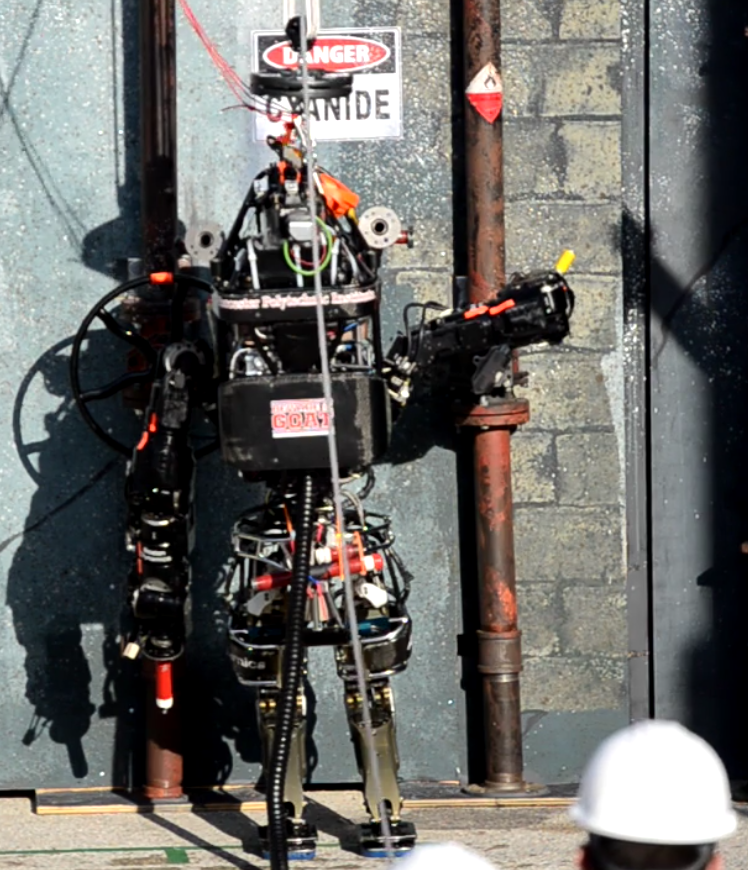
\includegraphics[scale=0.2]{images/turn_valve.png}
  \end{center}
  \caption{Robot in front of valves. Both shoulders right in front of each valve.}
\end{wrapfigure}
The first problem to achieve the task is to step towards the valve. The operator must activate the point cloud feedback on the computer, and position a marker on top of what looks to be a valve on the collection of dots. With the marker in place, it gives the operator the position of where the feet must be placed wherever the robot is going to use the left hand, or the right hand, to operate the valve. 

As demonstrated by a kinematic reachability study performed by MIT, the robot seems to have the best range of motion right in front of it's shoulder. \cite{mitaffordance} 

The initial approach to complete this task was to use the Boston Dynamics motion controller, and perform the motion by solving for different positions using MoveIt!, but this approach quickly presented several problems, such as when solving for the 6-DoF arm, it would only occasionally find a solution, and it was unable to complete the full motion. Another problem arose when using the 6-DoF arm + 3-DoF back joints, MoveIt! would use the back joints way too much for the motions and cause unpredictable behaviour. There was no direct way of limiting the motion of specific joints through MoveIt!.

The final method used the Carnigue Mellon's Full-body controller. This allowed a human operator to choose in which quadrantal direction to move the end-effector, analyze the force being applied to the hand, and move the hand in which ever direction necessary. 

\subsection{Results}
The task could be completed pretty robustly, and during the DRC trials, it was complete without any faults in 29 minutes, with only one minute to spare. 

\subsection{Conclusion and Future Work}
It is feasible to perform the entire task autonomously. The valves are easy objects to recognize, since they are big extrusions from the wall, and the motions are fairly simple. 

\section{DRC Wall}
\begin{wrapfigure}{r}{0.3\textwidth}
  \begin{center}
    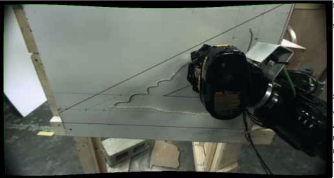
\includegraphics[scale=0.5]{images/drilling2.png}
  \end{center}
  \caption{The front camera vision of drilling the wall}
\end{wrapfigure}
For the Wall task the robot must use a single handed cordless rotary tool with an on/off switch to cut and remove a prescribed triangular shaped piece from a wall. The wall material will be 0.5 inch thick drywall. The three vertices of the right triangle will be 6 inches diameter circles. The edges connecting the vertices will be 6 inches wide. The vertical edge will be 12 inches long, and the horizontal edge will be 24 inches long. The bottom of the triangle will be 36 inches above the ground. \cite{walltask}

\subsection{Approach}
Performing the Wall task was a bit of a challenge for two reason: \begin{inparaenum}[\itshape a\upshape)]
\item Being able to progress the power-tool trigger and 
\item having the mobility to cut the wall in one motion. \end{inparaenum} 

\subsubsection{Picking up the drill}
Finding the drill on the point cloud is mostly a trivial task for the robot operator. Specially since the hight of the table was given in the task description. On the robot walked to the table, DARPA gave the option to choose one of two drills:

\begin{itemize}
\item One Dewalt DCD980M2 cordless drill: The robot must grasp the drill and squeeze the trigger to maintain the drill on. The drill also has a side handle to help with maneuverability. The problem with this drill is that the Robotiq hand had no way to firmly grasp the handle and press the trigger at the same time. The shape of the handle would cause the hand's middle finger on the back side of the drill to push out the front finger out of the trigger whenever any kind of firm grasp was applied. 

\item Dewalt DC550 cordless drill: It has an on/off switch. It was quite easy to grasp and operate, but pressing the small button on the base of the drill was quite difficult with the robot's large hands. The most reliable solution that we found is to shake the drill after grasping it, and add an extension on the hand such that it presses on the ON button.  Since the battery asymmetrical, the heavier side always slowly moves towards the ground, and causes the ON button to fall onto the hand's added extrusion. 
\end{itemize}

We found that the DC550 was the best option. The drill also provided a much wider range of motion while moving the arms. 

\subsubsection{Cutting the wall}
Once the drill was turned on, the robot would walk towards the wall and position his right shoulder parallel to the bigger side of the triangle. Once the robot start cutting the wall, the two main issues were:  \begin{inparaenum}[\itshape a\upshape)]
\item Ensuring that the drill bit was far enough in the wall, and  
\item The battery of the drill was not drained. \end{inparaenum} 

DARPA promised the teams that the drill would be fully charged at the beginning of each run, but during one practice run before the competition, the battery ran out before finishing the first cut. The controller quite reliability able to perform the entire motion without having to take a step. The operator would tell the robot to move one centimeter at a time in a direction, and monitor the hand forces applied.  

\subsection{Results}
During the competition, the operator made an error in the robot operation mode. Each of the hands has the option to either move the hand by setting a position relative to the floor, setting fixed joint values. While the right hand, which is operating the drill, is used with relative positions, the left hand is left at fixed joint values, not to add additional constraints to the kinematics. 

The left hand was accidentally turned on into relative positions, and since there were no graphical feedback about the operation of each hand, the operator was unable to determine why the robot was unable to move as freely as necessary to cut the wall. On an attempt to reset the controller while the robot was still running to fix the unexpected behaviour, the robot fell, having to reset the task. 

On the second attempt, the team only had about 10 minutes left to perform the task, and while it was possible to grab and turn on the drill, the robot was unable to finish the first cut in time.

\subsection{Conclusion and Future Work}

The approach of the task was solid and presented little issues most of the times. Due to the operator stress, and lack of visual cues about the robot state, the task was not completed. It is also feasible to perform the task autonomously with the current technology and resources. 

\chapter{Robust Dynamic Programming}
Model based optimal control is a powerful tool but relies heavily on the accuracy of the system model, which is not a trivial task to derive. There are many parameters involved, such as friction, sensor readings, calibrations, and the model may change over time due to wear, temperature, humidity, contact condition, and others.

Eric Whitman looks into using Multiple Model Dynamic (MMD) Programming, and uses the inverted pendulum swing-up problem to demonstrate the algorithm. \cite{eric_thesis}
 
By using the content provided in his thesis, the references, and example code, work on providing other students comprehensive guild on MMD for future students, we are looking at the different advantages, and shortcomings that comes with the algorithm.

Based on his previous work this paper aims to clarify the fundamental concepts of MMD and provide graspable examples. Furthermore, a faster running-time implementation using a General Purpose Graphical Processing Unit (GPGPU).

\section{Looking at a Problem}
To have a better understanding on how the algorithm works, we are going to look at the  inverse pendulum swing-up example, which consists of a motor attached to the end of pendulum, and the controller aims to bring the pendulum to an upright position by applying torques based on the current state of the system. 

The expected behaviour for the control law is to apply a torque equal to the direction the pendulum is swinging, such that more energy is added to the pendulum with each period, and when the pendulum finally has enough energy to perform a full rotation, apply a torque opposite to the movement such that the pendulum stops in an upright position.  

Since our interested is in solving a variety of dynamic programming problems, we are going to look at a more generic solution that discretizes the whole state of problem, and attempts to find a adequate policy to reach the desired goal.

We are going to assume that the pendulum has a length, $L=1m$, and a weight, $m=1kg$, and the world has a gravity $g=9.81\frac{m}{s^2}$. The pendulum has a 2-dimensional state space, $\theta$, the angle of the pendulum relative to the up position, and $\omega$, the current velocity in radians per second. There is only a one-dimension action space, $\tau$, the force of the motor can apply, and limit it at $\pm 1.5 \frac{N}{s}$.

The pendulum dynamics can be described by:

\begin{equation} 
\dot{\omega} = \frac{mLg \cdot sin(\theta) + \tau}{mL^2}
\end{equation}

Define the state space as $x=\{\theta, \omega\}$, and the action space to be $u=\{\tau\}$. We define the pendulum to be pointing up at, $\theta = 0$, and we are optimizing the pendulum to reach $\theta = 0$, with zero velocity, $\omega = 0$, using the minimum torque necessary. We define the cost function be to $L$:

\begin{equation} 
L(x,u) = \theta^2 + 0.5 \cdot \omega^2 + \tau^2
\end{equation}

And we want to minimize the total cost function, C, given by the integral: 

\begin{equation} 
C = \int L(x,u) dt
\end{equation}

We discritize the state space of the pendulum by assuming $\theta \in  (-\pi,\pi)$, and $\omega \in (-10,10)$, and define a 2-dimensional increments of 0.016 radians, and 0.022 radians/second, giving us a table of 360,000 states. We also assume a time step of T=0.003 second delay between each action, and sensor reading of the current pendulum state. We define the iteration function:

\begin{equation} 
x_{k+1}(u) = 
\begin{bmatrix}
\theta_{k+1} \\
\omega_{k+1}
\end{bmatrix}
=
\begin{bmatrix}
\theta_{k} + T \cdot \omega_{k} + \dot{\omega} \cdot T^2 \\
\omega_{k+1}
\end{bmatrix}
\end{equation}

For each state of the pendulum, we define two elements, the value $V(x) = {v}$, and let the initial value of $V(x)=0$ for all $x$, and the policy $U(x)={\tau}$, and let the initial value for all states be equal to 0. For optimizing the policy, we guess a random torque, $\tau'$, for every state in the grid, x, and define:

\begin{equation} 
V'(x) = C(x,u) + \gamma V(x_{k+1}(\{\tau '\}))
\end{equation}

And if $V'(x)<C(x,u) + \gamma V(x_{k+1}(U(x)))$, we let $V'(x)$ and $U(x)={\tau'}$.

We run the previous operation on all states of the grid for an uncertain number of times. For this particular program, running this optimization for 1000 iterations is sufficient for making the pendulum converge to the desired goal state, but it can also be noted that running for 10000 times generates a more torque efficient solution.

The problem is simple enough with the single-link pendulum case, but when extra links are added to the pendulum, such as the double-link pendulum, the problem becomes increasingly difficult to solve, but the algorithm can still find a sub-optimal policy with the modifications of redefining the state space, action space, and the iterate function.

\section{Running through an example}

To better comprehend how this problem is solved, let’s take a first iteration from a single discrete point in the grid. Suppose we are analyzing the $\omega_0=\frac{\pi}{2}, \omega_0=1 rad/sec$, and since we are in the first iteration, our current policy is $\tau_0=0$. If we keep the current torque, we find that the next step is:
	
\begin{equation} 
\dot{\omega_0} = \frac{1 \cdot 1 \cdot 9.81 \cdot sin(\frac{\pi}{2})+0}{1 \cdot 1^2} = 9.81
\end{equation}

\begin{equation} 
\begin{bmatrix}
\theta_{k+1} \\
\omega_{k+1}
\end{bmatrix}
=
\begin{bmatrix}
\theta_{k} + T \cdot \omega_{k} + \dot{\omega} \cdot T^2 \\
\omega_{k+1}
\end{bmatrix}
=
\begin{bmatrix}
\frac{\pi}{2}+1 \cdot 0.003 + 0.5 \cdot 9.81 \cdot 0.0032 \\
1 + 9.81 \cdot 0.003
\end{bmatrix}
=
\begin{bmatrix}
\frac{\pi}{2}+0.003044145 \\
1.02943
\end{bmatrix}
\end{equation}

And we can now discover the current value of $V(x)$ to be:
\begin{equation} 
V(x) = C(x,u) + \omega V(x_{k+1}(\{\tau'\})=(\theta^2+0.5 \cdot \omega^2 + \tau^2)+1 \cdot 0 = 2.6032705
\end{equation}

Since this is the first iteration of this equation, the second term of the value equation is 0. Now suppose that we guess $\tau=1$, and find the new state to be:


\begin{equation} 
{x'}_1 = 
\begin{bmatrix}
\frac{\pi}{2} + 0.003048645 \\
1.03243
\end{bmatrix}
\end{equation}

We find the new value of
\begin{equation} 
V'(x) = 2.6062750
\end{equation}

Since $2.6032705 < 2.6062750$, we learn that we are applying a torque in the wrong direction, and it is better to let gravity pull on the pendulum instead of applying addition torque, and keep the value, $U(x)={0}$. Now suppose we guess $\tau = -1$, we find that 
\begin{equation} 
{x'}_1 = 
\begin{bmatrix}
\frac{\pi}{2} + 0.003039645 \\
1.02643
\end{bmatrix}
\end{equation}
With the value
\begin{equation} 
V'(x) = 2.6002660
\end{equation}

Since $2.6032705 > 2.6002660$, we change the value $U(x_0)={-1}$. Giving a new optimal torque to apply at that point.

It is important to notice the optimal torque may completely change directions throughout the iterations due to the value of the neighbours changing. (Further details with the video)

\section{Analysing this solution}
The algorithm is far from being real time, since for the single-link pendulum case, on an 8-core CPU at 2.8 GHz, takes about 4 seconds for each iteration, and about 1 hour for the 1000 iterations, but it does generate very robust policy tables.

On the following plot we show the policy of 10,000 iterations running against a pendulum, position of the pendulum relative to the up position, starting at pi, pointing down, and with 0 velocity. It is interesting to see that the policy follows similar to a bang-bang controller, using near maximum torque on both directions, until the system has enough energy to reach the necessary solution. 

The following plot demonstrates the value and the policy values of the pendulum swing-up solution. The X-axis is the velocity of the pendulum, while the Y-axis is the current position of the pendulum. 

Figure~\ref{fig:pendulum_plot} states that as the pendulum starts at $[\pi, 0]$, starting with the pointing down, with no velocity, and on the highest value on the value plot. Over time, the pendulum will travel down the apply torque and gain velocity over time, up to the point that the pendulum will reach the lowest value on the plot. 

Figure~\ref{fig:pendulum_time_plot} shows the position, velocity, and torque being applied at any moment on the pendulum. Even with 1,000 iterations the system was able to find a method in which the position converges to 0, when the pendulum is pointing up, but one can also see that during the last 20 seconds, the line contains quite some noise.

Lastly, on Figure~\ref{fig:pendulum_plot2} shows the paths of pendulum. Each red line represents the start configuration of a pendulum, and stops when they go outside of the plot, or reaches the desired position at $[0,0]$. It was surprising to learn that on the top-right corner, when the pendulum has some momentum and is pointing down, they do not all converge exactly to the same path, but are rather somewhat parallel to one another.

\begin{figure}
\begin{center}
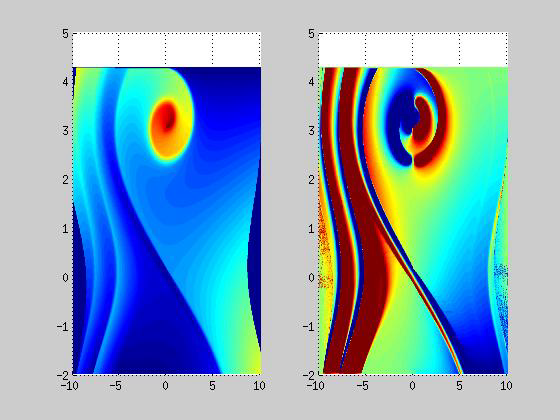
\includegraphics[scale=0.7]{images/DDP.png}
\caption{Plot showing the value and policy of a pendulum swing up}
\label{fig:pendulum_plot}
\end{center}
\end{figure}

\begin{figure}
\begin{center}
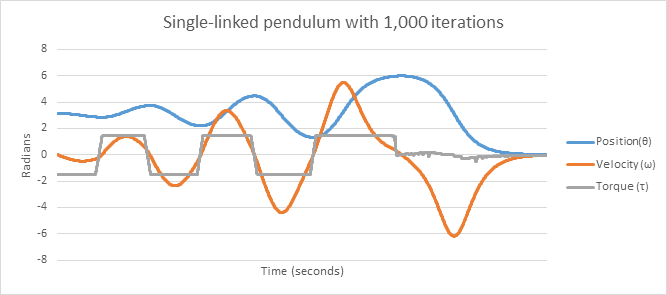
\includegraphics[scale=1.0]{images/Pendulum_time.png}
\caption{Position, velocity, and torque of pendulum over time}
\label{fig:pendulum_time_plot}
\end{center}
\end{figure}

\begin{figure}
\begin{center}
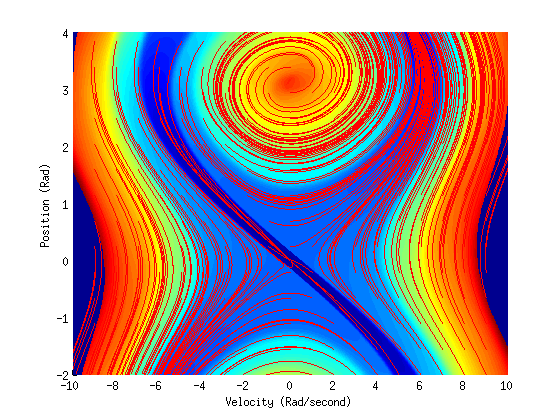
\includegraphics[scale=0.8]{images/direction_lines.png}
\caption{Paths that pendulum would follow given any start position}
\label{fig:pendulum_plot2}
\end{center}
\end{figure}




\section{CUDA}

To first understand why using a GPGPU is a faster tool that fits to solve this problem, we must first take a look at the history of how games and GPUs, and how the computing model of GPU’s fits this problem.

The principles of a modern game rendering have not changed much since the beginning; A list of triangles in 3d space are transformed, projected into a plane, and then each pixel is rendered with the color of the closest triangle. The three major steps in the rendering pipeline involves:

\begin{enumerate}
\item Vertex processing: Each vertex in a model is moved into a new position by transformation matrices and weights.
\item Rasterization: Processing each of the triangles in the screen region, and calculating what the closest triangle in each pixel is.
\item Fragment shading: Determined the color of each pixel based on the closest triangle. (The coordinates of the closest triangle is passed into the fragment shader)
\end{enumerate}

While the second step is usually done by hardware, hidden away from developers, the main aspects of the first and third step is that each vertex and pixel can be completely independent of one another and can be programmed by C-like programs, called shaders. Due the popularity and profitability

of game companies, this gave incentives for companies to develop dedicated hardware that process each of the points as quickly as possible.

Until 2001 developers could only use shaders that were pre-programmed into the hardware, and then Direct3D 8 \cite{wiki:direct3d} gave developers the option to program custom shaders that run in the hardware.

The main drive for GPU development was for computer graphics, but using some technique, one could speed up large linear algebra processing using storage through image textures. \cite{Goeddeke:2005:GBM}

For example, OpenGL could be used to perform the multiplication of two 256 by 256 matrices. In this case, three texture buffers would be created inside of the GPU, each of the size of the matrix, and two of them would be loaded with the read-only input matrices values from the main computer memory, while the other one would be used as a render texture. When the fragment shader runs over all the pixels of the render texture, the user defined program would read the necessary values from the other two matrices and render the corresponding output value. 

Later during 2007, NVIDIA released CUDA, a general purpose computing standard that would allow developers to create GPU based software, and later on 2008, the open source community followed with OpenCL. While OpenCL and CUDA follows the same principles as fragment shaders, it also opened doors for other applications, such as atomic operations, thread syncing, memory barriers, and others.

\section{Applying DDP with CUDA}
Since a new improved torques can be found in parallel with other points, we can run the Dynamic Programming Algorithm using CUDA.  We initialize the process by allocating two memory buffers in the device, and reset all of the values to 0.  We create a CUDA kernel, which takes an identification number, input memory buffer, and compares the current policy with a new random policy, and stores the result on an output buffer. 

We then swap the input buffer with the output buffer and repeat the process for the given number of iterations.  The process otherwise is equivalent to the CPU’s counterpart, but instead of taking up to 1 hour to complete, the GPU process only took 2 minutes. 

The limitations with using a GPU for this kind of process is a more limited memory space, while it can be relatively cheap to buy more computer RAM, or allow the computer swap memory into a solid state drive, the GPU is limited to only to the memory available on the device, and even devices top of the line today, such as the NVIDIA Tegra 4, only provides 4GB of memory. 

\section{Results}
The results of the algorithm were never applied in a real system, and the generated value and policy for the GPU and CPU were essentially identical. Presenting sensor noise and other real-life factors into a simulation, we can still see that the system can still perform under inaccurate actuation. \cite{eric_thesis}

\section{Conclusion}
Dynamic Programming still has the Curse of Dimensionality, the dimensions of the project can be scaled down to fit into a manageable set, and since the data storage is rather comparably cheap, the information could be stored in disk for later retrieval. Furthermore, with the help of CUDA, specific sections of the grid could be recalculated with finer detail in real time when needed. 

The Pendulum-Swing problem has been solved many times before, but with this type of solution, the problem can be extended to higher dimensions, and it only requires an linearised model of the system. The algorithm could be easily extended to take a double, triple, or any given number of links pendulum.  

\section{Future Work}
This problem could be extended into looking at different end-effector positions for Atlas. One could generate a table of all feasible end-effector positions, and find paths on how to travel from one position to another while minimizing change in the center of mass deviation from the support polygon.

\chapter{Future Work}

The WPI-CMU team performed well on the DRC trials. Regardless, due to the time constraints a lot of the code was built in a hurry, and without a proper structure. It is important to create a strong code base that can evolve over the years, and adapt to future challenges. An important aspect of having a strong base is being able to perform experiments, and build upon previously developed work. A lot of emphasizes after the DRC trials was directed on refactoring the code base, and there is still a long way to go.

%Science is the process of having a hypothesis, creating an experiment, and analysing the results.  

As mentioned earlier in the paper, there is plenty of research in the subjects of object detection, manipulability, planning, and others, but it is a different challenge to be able to adapt all this work into a single code base, and be able to perform experiments, while using data from all the different aspects of the robot. 

New goals for the team should focus on tools that can be reused and extended at later times. For example, with the step planner, a developer should be able to instantiate a new planner either with simulation, or the real robot, and have access to modify each of the steps. At a later time, a team can extend the initial step planner to automatically generate all of the steps, but should still leave the option to use the old planner.

A great library is one that allows the user to choose the tools to complete their task, and modify one of the steps as necessary, and it is a difficulty that research does not often present to students, since students are usually only required to use a library, instead of developing on the library itself. 

The ultimate goal of this project would be to perform all the tasks a human is able to do, but developers must be able to break down the complex tasks into simpler steps, and understand the difficulties that comes before moving into solving a generalized case. 


%this is an example how to include a figure in eps-format. Refer to 
%latexguide.ps for more help.
% this example loads the file /figures/mychart.eps

%\begin{figure}[htb]
%  \begin{center}
%    \includegraphics[width=5cm]{mychart.eps}
%    \caption{A picture in \LaTeX}
%    \label{fig:my_first_figure}
%  \end{center}
%\end{figure}



\bibliography{referencex}
\bibliographystyle{plain}
% not just one chapter, but as many as needed to explain the results

\nocite{*}
%%%%%%%%%%%%%%%%%%%%%%%%%
\end{document}

